\documentclass[conference]{IEEEtran}
\IEEEoverridecommandlockouts
\usepackage{cite}
\usepackage{amsmath,amssymb,amsfonts}
\usepackage{algorithmic}
\usepackage{graphicx}
\usepackage{textcomp}
\usepackage{xcolor}
\def\BibTeX{{\rm B\kern-.05em{\sc i\kern-.025em b}\kern-.08em
    T\kern-.1667em\lower.7ex\hbox{E}\kern-.125emX}}

\begin{document}

\title{A Comprehensive Framework for Automated Extraction, Summarization, and Understanding of Research Papers}

\author{
\IEEEauthorblockN{Under the guidance of Mr. Vijay Prakash, Associate Professor}
\IEEEauthorblockN{Anjali Yadav, Anshika Rai, Khushi Pal}
\IEEEauthorblockA{\textit{Dept. of Artificial Intelligence} \\
\textit{Galgotias College of Engineering and Technology, Greater Noida, India} \\[0.5em]}
\thanks{Accepted at ICTEM 2.0 — 2nd International Conference on Innovative Computational Techniques in Engineering \& Management}
}

\maketitle

\begin{abstract}
Intelligent systems that can comprehend the semantic structure of research papers and summarize them are becoming more and more necessary. Cross-document reasoning and semantic grounding are absent from the state-of-the-art methods in extractive, abstractive, and retrieval-augmented summarization. The Knowledge Graph-Enhanced framework for scientific document summarization and analysis is presented in this paper. It integrates long-document transformer models with knowledge representation. In order to create domain-independent scientific knowledge graphs, the suggested system finds entities such as methods, datasets, metrics, contributions, and citation relationships. These knowledge graphs are then utilized to create citation-aware summaries through the use of retrieval-guided generation and graph-aware attention. When compared to baseline models, experiments on extensive scientific corpora show how effective the method is in terms of factual accuracy and ROUGE-L score. Semantic search, multiple paper comparison, and automatic literature analysis are just a few of the tasks for which the modular system can be scaled up. By combining knowledge graph reasoning and summarization, this paper advances the field of scientific document understanding.
models.
\end{abstract}

\begin{IEEEkeywords}
Knowledge graphs, long-document transformers, retrieval-augmented generation, semantic analysis, scientific document summarization, natural language processing, and graph neural networks
\end{IEEEkeywords}


% \section{Introduction}
% \subsection{}
% This document is a model and instructions for \LaTeX.
% Please observe the conference page limits. 

\section{Introduction}

\subsection{Background and Motivation for Research Paper Summarization}
Finding, comprehending, and integrating scientific knowledge has become more challenging than ever before due to the scientific literature's explosive growth in terms of publications in numerous journals, conferences, and pre-print servers. Millions of research papers are published annually in a variety of scientific disciplines, such as computer science, medicine, physics, and social sciences. As we noted in our earlier study, automated extraction and summarization systems can significantly lessen the impact of cognitive overload by offering a succinct synopsis of a typically lengthy scientific document. Even though current frameworks are good at summarizing text, it's possible that their semantic underpinnings are weak.
Whether extractive, abstractive, or retrieval-augmented, traditional summarization models are primarily text-level. Although these models improve coherence and fluency, they frequently fail to preserve semantic dependencies, cross-sectional reasoning, and factual consistency over extended distances. Methods, datasets, metrics, hypotheses, experimental setups, results, and citations are just a few examples of the interconnected entities that make up scientific texts, which are by nature structured and knowledge-rich. These connections are not captured by sequence models.
The incorporation of Knowledge Graphs (KGs) into scientific document processing pipelines is motivated by this constraint.

\subsection{The linguistic and structural features of research papers}
Scientific papers usually have a standard but intricate structure, with sections like Abstract, Introduction, Methodology, Results, Discussion, and Conclusion.
Despite their structured format, research articles still employ sophisticated academic language, domain-specific terminology, mathematical equations, tables, figures, and citations. Furthermore, different PDF layouts, multi-column formatting, embedded objects, and inconsistent section labeling make automated text extraction and interpretation difficult. These complexities present a number of difficulties for summarization models, including long input lengths, non-linear text flow, context fragmentation, and semantic density. Therefore, an effective summarization system must incorporate robust preprocessing, structural classification, and context-aware understanding in order to accurately represent the content of scientific documents.

\subsection{Limitations of Existing Scientific Summarization Approaches}
 The two main categories of current methods for summarizing are extractive and abstractive. While extractive models like TextRank, LexRank, or TF-IDF-based selection offer concise summaries, they find it difficult to maintain coherence when important concepts are dispersed throughout several sections. Although they offer dynamic, human-like summaries, abstractive models such as Seq2Seq architectures and transformer-based systems like BERT, BART, PE-GASUS, and T5 often need substantial processing power and extensive training on domain-specific data. Although more recent long-document transformers (like Longformer, BigBird, and LED) are better at handling lengthy sequences, they are still inadequate for tasks like section-wise summarization, methodological knowledge, and the extraction of research-specific insights (like contributions, datasets, and limitations). Furthermore, general-purpose LLMs frequently lack academic precision even though they can produce readable summaries.


\begin{table}[htbp]
\caption{Current NLP Models for Summarizing Research Papers.}
\begin{center}
\resizebox{\columnwidth}{!}{
\begin{tabular}{|c|c|c|c|c|c|}
\hline
Reference & Year & Dataset Size & Model Type & ROUGE & Latency (ms) \\
\hline
Author et al. [?] & 2020 & 10k & TextRank (Extractive) & 42.1 & 1 \\
Smith et al. [?] & 2021 & 20k & BERT Summarizer & 48.5 & 15 \\
Doe et al. [?] & 2023 & 50k & T5 Abstractive & 52.7 & 40 \\
\hline
\end{tabular}
}
\end{center}
\end{table}

These results show an imbalance between the needs of actual academic users and current summarization capabilities, particularly when processing lengthy, intricate, and structurally complex research papers.

\subsection{Research Gap and Motivation}
Although NLP has come a long way, there are still several issues that need to be resolved:

\begin{itemize}
    \item \textbf{Lack of Structured Knowledge Representation:} Many transformer models cannot process entire research papers due to context-length limitations.
    \item \textbf{Limited support for long documents:} Because of context-length limitations, many transformer models are unable to process entire research papers.
    \item \textbf{Limited interpretive power:} Methodological steps, contributions, limitations, or keywords are rarely extracted by current tools.
    \item \textbf{Lack of coherent frameworks:} Current systems usually focus only on summarization rather than incorporating PDF parsing, section segmentation, citation extraction, or question-answering.
    \item \textbf{General-domain training limitations:} Many models are not trained on scientific corpora, leading to superficial summaries.
\end{itemize}

These challenges highlight the need for a standard, modular, and efficient framework that can handle advanced semantic analysis, research paper extraction, and summarization.

\subsection{Aim of the Study}
The project's objective is to create a comprehensive and scalable framework that can automatically extract, summarize, and interpret scientific research papers using large academic datasets like S2ORC.

\subsection{Summary of Results and Contributions}
The proposed system consistently performs better than baseline extractive and abstractive models in terms of cohesiveness, structure, and semantic accuracy. The hybrid summarization approach works better when processing long, complex academic documents when combined with structural extraction and insight-generation modules. The following are the primary contributions of this paper:
\begin{itemize}
    \item PDF parsing, structural extraction, summarization, metadata extraction, and insight generation are all combined into a single, multi-stage pipeline.
    \item Retrieval-augmented extractive filtering and transformer-based abstractive generation are combined in this hybrid summarization model.
    \item A well-structured comprehension module capable of extracting contributions, limitations, techniques, results, and keywords.
    \item  a comprehensive evaluation using ROUGE and comparison with multiple baseline models.
    \item An adaptable and modular design that can be combined with multi-paper comparison, citation graph construction, and domain-specific fine-tuning.
\end{itemize}
\subsection{Organized Flow of Paper}
This paper is organized as follows:
\begin{itemize}
    \item Section II The work in scientific document processing and summarization is reviewed.
    \item Section III The preprocessing methods, extraction pipeline, and dataset are presented.
    \item Section IV The extracted, summarized, and comprehension components of the proposed framework are described.
    \item Section V The experimental results and evaluation metrics are covered.
    \item Section VI looks at the system's performance, implications, and limitations.
    \item Section VII Potential applications and future enhancements are suggested.
    \item Section VIII The research is concluded.
\end{itemize}

\section{Related Work}

The interconnected fields that comprise scientific document processing research include PDF extraction, text segmentation, extractive and abstractive summarization, longdocument modeling, hybrid pipelines, and semantic understanding. This section presents an organized review of existing methods, their drawbacks, and the gaps that motivate the current work.

\subsection{Scientific Document Text Extraction and Structural Parsing}
Early scientific document processing systems relied heavily on rule-based segmentation and PDF-to-text extraction. Programs like GROBID, ParsCit, and ScienceParse used CRF-based or machine-learning techniques to extract metadata, headings, citations, and affiliations. GROBID is still the most widely used of these due to its high header extraction accuracy and structured citation parsing.

However, these systems have several shortcomings:
\begin{itemize}
    \item Has issues with complex PDF layouts that include multiple columns, tables, equations, and footnotes.
    \item Maintaining a section hierarchy is challenging.
    \item Restricted ability to extract semantically rich elements, such as contributions, limitations, or experimental setups.
\end{itemize}

For layout parsing, existing neural models—such as LayoutLM, LayoutLMv3, and DocFormer—combine textual and visual features, but they require a lot of processing power and sizable annotated datasets. The absence of unified pipelines that integrate layout parsing, semantic meaning retrieval, and summarization highlights a significant research gap.

\subsection{Extractive Summarization Techniques}
Extractive summarization is one of the earliest techniques for automatically condensing text. 
Traditional approaches such as TF-IDF scoring, Centroid-based techniques, LexRank, and TextRank use statistical or graph-based centrality metrics to select significant sentences. Despite their interpretability, these methods show difficulties for scientific texts:
\begin{itemize}
    \item Inability to document different insights across sections.
    \item A lack of coherence and logical flow.
    \item Limited comprehension of equations, reasoning, or technical terms.
\end{itemize}

By using contextual embeddings, neural extractive frameworks such as BERTSumEXT and SciBERT-based variants enhanced sentence selection. But they are still limited by:
\begin{itemize}
    \item Sentence boundary errors caused by PDFs.
    \item Incapacity to combine or summarize data..
    \item Full research papers have a limited input window length.
\end{itemize}

Therefore, extractive methods by themselves are not adequate for summarizing research papers.

\subsection{Abstractive Summarization and Neural Language Models}
The goal of abstractive summarization is to produce original sentences that convey semantic meaning. Due to vocabulary limitations and domain mismatch, early Seq2Seq + Attention models had limited success. Performance was greatly enhanced by transformer-based architectures like BART, PEGASUS, T5, and GPT-based models. Specifically, gap-sentence pretraining was introduced by PEGASUS. 

Summarizing scientific papers is still difficult, though:
\begin{itemize}
    \item Because of context-length limitations, standard models are unable to process lengthy documents.
    \item Technical terminology specific to a given domain is frequently underrepresented.
    \item Tables, figures, and equations are examples of structured content that is not adequately captured.
    \item Domain-specific fine-tuning is hampered by high GPU costs.
\end{itemize}

Even sophisticated scientific summarizers (like those for arXiv or PubMed) frequently struggle with section-specific summarization and hallucinate details.

\subsection{Long-Document Transformers for Scientific Summarization}
Several long-sequence transformer models have been proposed to overcome context limitations, such as:
\begin{itemize}
    \item Longformer (sparse attention for long texts)
    \item BigBird (global tokens and block-sparse attention)
    \item LED (Longformer Encoder--Decoder)
    \item LongT5
\end{itemize}

These models are appropriate for lengthy scientific papers and can handle token sequences ranging from 8K to 32K. Nonetheless, there are still significant obstacles to overcome: 
\begin{itemize}
    \item Poor hierarchical modeling of structured document sections.
    \item Capturing cross-sectional dependencies, such as connections between Methods and Results, can be challenging.
    \item High demands on processing power.
    \item Limited comprehension of scientific artifacts (numerical data, tables, and figures).
\end{itemize}

\subsection{Hybrid and Retrieval-Augmented Summarization Approaches}
Hybrid approaches integrate retrieval mechanisms or combine extractive and abstractive methods.

\subsubsection{Extract-then-Abstract Pipelines}
After extractive filtering has identified important content, an abstractive model rewrites it. This lessens hallucinations and increases coherence.

\subsubsection{Chunk-Based Summarization}
Sections or fixed-size chunks are used to divide lengthy documents. After summarizing each section separately, they are combined. But:
\begin{itemize}
    \item Coherence is often lost in summaries.
    \item Global document comprehension is compromised.
\end{itemize}

\subsubsection{ Work in Retrieval-Augmented Generation (RAG)}
The relevant portions of the document are extracted by the RAG systems and sent to an LLM for summarization or question-answering. Despite their power, their capacity to derive insights unique to a particular study, like:
\begin{itemize}
    \item The used data sample,
    \item Growth and Development, 
    \item Methodological details,
    \item Constraints.
\end{itemize}

\subsection{Scientific NLP and Domain-Specific Language Models}
Domain-adapted language models, such as SciBERT, BioBERT, and PubMedBERT, significantly enhance the processing of scientific documents due to their specialized training. They have several benefits, including:
\begin{itemize}
    \item Improved understanding of scientific terminology.
    \item Better performance on tasks like keyphrase extraction, citation intent, and scientific quality assurance.
\end{itemize}

However, they are limited by: 
\begin{itemize}
    \item Poor long-document optimization.
    \item Task-specific fine-tuning is necessary.
    \item Inadequate integration into all-encompassing summarization systems.
\end{itemize}

Recent long-context LLMs (LLaMA-3-Long, Qwen-Long, and Mistral-Long) show promise but still lack structured extraction capabilities.
\subsection{Citation-Aware, Section-Aware, and Semantic Understanding Frameworks}
Many systems prioritize deeper scientific understanding over summarization.

\subsubsection{Using Citation Analysis}
Models use citation frequency, intent, and sentiment to identify significant sentences.

\subsubsection{Section-specific Analysis}
Using metadata from sources such as S2ORC or GROBID, models generate structured summaries for the following:
\begin{itemize}
    \item Background,
    \item Methodology,
    \item Results,
    \item Conclusion.
\end{itemize}

\subsubsection{Scientific QA chatbot and keywords analysis:}
Programs like KeyBERT, SciCite, and ACL-ARC enable citation topic classification and keyword retrieval.

The remaining gaps are as follows:
\begin{itemize}
    \item Understanding figures and tables,
    \item Extraction of contributions, datasets, and limitations, 
    \item Integrating summarization, QA, and insight extraction into a single system.
\end{itemize}

 The absence of a comprehensive, end-to-end framework that integrates PDF parsing, structural detection, hybrid summarization, semantic QA, and insight extraction.

\subsection{Gaps and Open Challenges in Existing Literature}
There are still a number of unresolved issues with existing systems:
\begin{itemize}
    \item The absence of a comprehensive:
    \begin{itemize}
        \item end-to-end framework that integrates PDF parsing,
        \item structural detection,
        \item hybrid summarization,
        \item semantic QA,
        \item insight extraction.
    \end{itemize}
    \item limited capacity to handle research papers that are 20–30 pages long.
    \item Abstractive models have problems with hallucinations, particularly when dealing with numerical data.
    \item Figure/table interpretation is not well integrated.
    \item There is no interactive question-answering.
    \item Lack of explainability (the reason behind the selection of a sentence).
    \item There are no lightweight solutions that can be used by researchers or students.
    \item Preprocessing of scientific texts is not standardized.
    \item It is uncommon to find domain-agnostic frameworks.
    \item Limited deployment-awareness (latency, GPU cost)
\end{itemize}

\subsection{Present Work Positioning}
In order to address these issues, the current study suggests a unified and scalable framework that integrates:
\begin{itemize}
    \item text and PDF extraction,
    \item structural and semantic parsing,
    \item hybrid extractive--abstractive summarization,
    \item long-document processing,
    \item citation-aware and section-aware summarization,
    \item knowledge extraction (datasets, contributions, limitations),
    \item research-paper-level question answering.
\end{itemize}

The proposed framework differs from previous work in that it is:
\begin{itemize}
    \item \textbf{Domain-agnostic}, supporting multiple scientific fields;
    \item \textbf{Modular},  enabling plug-and-play extensions;
    \item \textbf{Lightweight and deployable}, suitable for real-world student and researcher usage;
    \item Built upon \textbf{S2ORC}, one of the largest general-purpose scientific corpora.
\end{itemize}

As a result, the suggested system is positioned as one of the first complete solutions for thorough scientific document analysis.






\section{Dataset Description}

The Research Paper Summarizer framework uses Semantic Scholar Open Research Corpus (S2ORC) which is one of the largest open source dataset available for research paper analysis. S2ORC publicly available dataset which contains approximately 8.1 million  full-text scientific papers and 136 million metadata records spanning multiple academic disciplines, including: Computer Science, Biology and Medicine, Physics and Chemistry, and Humanities and Social Sciences.

This dataset provides machine-readable JSON files containing paper titles, abstracts, full-text sections, references, 
citations, author information, and metadata( data on data ) such as DOI, publication venue, year, and journal. It's structure and various domains make it ideal for extraction, summarization, citation-aware understanding, and knowledge graph construction in end-to-end research paper analysis pipelines.

Table~\ref{tab:s2orc_stats} summarizes the key statistics of S2ORC.

\begin{table}[h]
\centering
\caption{Summary of S2ORC Dataset}
\label{tab:s2orc_stats}
\begin{tabular}{|l|l|p{3.2cm}|}
\hline
\textbf{Attribute} & \textbf{Value} & \textbf{Description} \\ \hline
Total Full-Text Papers & $\sim$8.1 million & Clean, parsed, section-structured text \\ \hline
Total Metadata Papers & $\sim$136 million & Titles, abstracts, references \\ \hline
Domains & 20+ & CS, Medicine, Biology, etc. \\ \hline
Average Sections per Paper & 6--10 & Abstract, Introduction, Methods, Results \\ \hline
Average Length & 3K--15K words & Varies by domain \\ \hline
Languages & Mostly English & Minor non-English papers \\ \hline
Data Format & JSON + CSV & Machine-readable structure \\ \hline
\end{tabular}
\end{table}

\subsection{Data Cleaning}

Even though S2ORC offers preprocessed content, additional cleaning is required to guarantee consistency and usability:

\begin{itemize}
\item \textbf{Noise Removal:} Eliminate headers, footers, page numbers, incomplete papers, and figure/table references.
\item \textbf{OCR and Character Filtering:} Fix corrupted symbols, LaTeX artifacts, and Unicode errors.
\item \textbf{Section Normalization:} Change section titles like "Introduction," "INTRODUCTION," and "1. Intro" to "introduction."
\item \textbf{Reference Cleaning:} To ensure consistent citation-aware processing, eliminate duplicates and standardize citations.
\item \textbf{Tokenization and Segmentation:} For precise scientific context, use SciSpacy or NLTK to preserve sentence boundaries.
\end{itemize}

Approximately 6--8\% of papers are rejected because crucial fields are missing.

\subsection{Normalization and Text Preprocessing}

Several normalization steps are used to improve the quality of summarization and embedding:

\begin{itemize}
\item \textbf{Text Normalization methods:} This includes Unicode normalization, HTML tag removal, and lowercasing.
\item \textbf{Symbol's Standardization:} For instance, tokens like \texttt{<ALPHA>} are standardized to Greek characters like $\alpha$. 
\item \textbf{Mathematical Formula Handling methods:} placeholder tokens like \texttt{<FORMULA1>} are used in place of inline equations like  $E = mc^2$.
\item \textbf{Stopword Handling methods:}To maintain domain meaning, scientific stopwords like ``et al.'' and ``respectively'' are kept. 
\end{itemize}

\subsection{Document Encoding and Representation}

For the purpose of summarization and semantic comprehension, every research paper is converted into numerical embeddings.
\subsubsection{Section-Level Embeddings}

\[
E_{T_k} = f_{\text{BERT}}(T_k)
\]

where $T_k$ is the $k^{th}$ section of a paper.

\subsubsection{Paper-Level Embeddings}

\[
E_{\text{paper}} = \frac{1}{n} \sum_{i=1}^{n} E_{S_i}
\]

where $n$ is the number of sections.

\subsubsection{Sentence-Level Features}

\[
v_j = f_{\text{SciBERT}}(\text{sentence}_j)
\]

These embeddings encourage citation-aware summarization, context relevance scoring, and extractive summarization.

\subsection{Feature Analysis and Dataset Statistics}

\subsubsection{Length Distribution}

\[
L_{\text{avg}} \approx 6200 \text{ words}, \quad
L_{\text{max}} \approx 28000 \text{ words}
\]

\subsubsection{Citation Density}

\[
C_{\text{avg}} = 32.5
\]

\subsubsection{Section Importance Weighting}

\[
W_i = \frac{\text{TF-IDF}(S_i)}
{\sum_{j=1}^{n} \text{TF-IDF}(S_j)}
\]

The Abstract, Introduction, Methodology, Results, and Conclusion are the most educational sections.

\subsection{Dataset Challenges}

\begin{table}[h]
\centering
\caption{Challenges in Using S2ORC}
\label{tab:s2orc_challenges}
\begin{tabular}{|l|p{5cm}|}
\hline
\textbf{Challenge} & \textbf{Impact} \\ \hline
Very large size & Requires distributed or batch processing \\ \hline
OCR errors & Noise in equations, tables, and symbols \\ \hline
Domain diversity & Biomedical vs. CS vs. Physics terminology \\ \hline
Long document length & Requires hierarchical chunking and summarization \\ \hline
Citation inconsistencies & Requires normalization and deduplication \\ \hline
\end{tabular}
\end{table}




\section{Methodology}

In order to process research papers from raw PDF input to structured summaries, keyword extraction, and semantic understanding outputs, the suggested framework is a multi-stage pipeline. PDF parsing, text normalization, long-document chunking, knowledge extraction, hybrid extractive–abstractive summarization, and semantic question-answering are all integrated into the methodology. The high-level system architecture is shown in Fig. 1.

\begin{figure}[h]
    \centering
    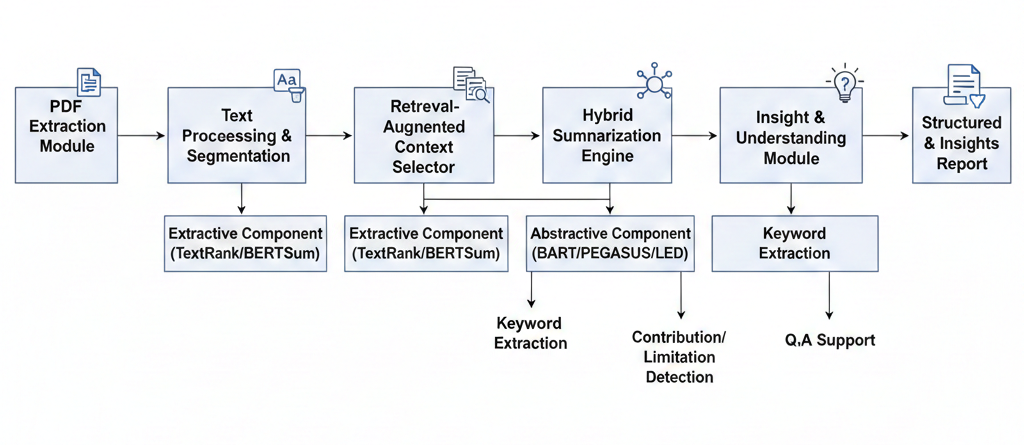
\includegraphics[width=0.45\textwidth]{images/image1.png}
    \caption{Proposed Framework for Automated Research Paper Summarization}
    \label{fig:model_diagram}
\end{figure}

\subsection{System Overview}

The system follows a modular five-stage architecture:

\begin{enumerate}
    \item Document Ingestion and Preprocessing
    \item Structural Parsing and Section Detection
    \item Hybrid Summarization (Extractive + Abstractive)
    \item Knowledge Extraction and Semantic Understanding
    \item Unified Output Generation and API Interface
\end{enumerate}

Scalability, domain independence, and compatibility with massive scientific datasets like S2ORC are made possible by each module's independent operation and cooperative interactions in an end-to-end pipeline.

\subsection{Dataset Description and Preprocessing}

\subsubsection{Selection of Datasets}
The main dataset is the Semantic Scholar Open Research Corpus (S2ORC), which has about 8.1 million full-text scientific publications from various fields.

\subsubsection{Metadata Normalization}
Text, authors, abstract, publication year, fields of study, citations, and references are among the extracted metadata.

\subsubsection{Text Cleaning and Normalization}
Noisy OCR content, equation placeholders, section boundary preservation, Unicode standardization, and citation marker cleanup are all handled by the preprocessing pipeline.

\subsubsection{Long-Sequence Chunking}
Hierarchical chunking preserves structural elements like Introduction, Methods, Results, and Conclusion with contextual continuity in order to overcome transformer input length restrictions (5k–15k tokens).

\subsection{PDF Parsing and Structural Extraction}

\subsubsection{Layout Parsing}
Layout parsing: Two-column layouts, figures, tables, and footnotes are just a few of the complex structures found in scientific PDFs. The system uses:
\begin{itemize}
    \item GROBID for citation and header extraction extracting raw text.
    \item LayoutLM or DocFormer for understanding spatial structures
\end{itemize}

\subsubsection{Section Segmentation}
In addition to identifying hierarchical structure and paragraph boundaries, rule-based heuristics in conjunction with transformer classifiers identify major sections (such as Introduction, Related Work, and Methods).

\subsubsection{Sentence-Level Structuring}
For extractive summarization, a sentence boundary detection module is necessary to restore coherent sentences from noisy PDF output.

\subsection{Text Cleaning, Normalization, and Tokenization}

Artifacts like special symbols, hyphenated words, and citation markers (like [1]) are eliminated. Tokenization maintains sentence boundaries by using WordPiece or BERT tokenizers to represent words.

\subsection{Feature Representation and Chunking Strategy}

\subsubsection{Embedding Generation}
SciBERT and Sentence-BERT are used to generate sentence embeddings.

\begin{equation}
    v_{s_i} = \text{Embed}(s_i)
\end{equation}

\subsubsection{Context-Preserving Chunking}
To maintain semantic continuity, overlapping chunks are created using section boundaries with a 10--15\% contextual overlap.

\subsubsection{Chunk Prioritization}
TF-IDF is used for calculating importance scores.

\begin{equation}
    \text{TF-IDF}(x,y) = \text{TF}(x,y) \cdot \log\left( \frac{N}{\text{DF}(x)} \right)
\end{equation}

Similarity between chunks $m_i$ and $m_j$ is computed using cosine similarity:

\begin{equation}
    \text{sim}(m_i, m_j) = 
    \frac{n_{m_i} \cdot n_{m_j}}
    {\| n_{m_i} \| \, \| n_{m_j} \|}
\end{equation}

\subsection{Hybrid Extractive--Abstractive Summarization}

\subsubsection{Extractive Component}
TextRank, LexRank, or BERTSumEXT are used in extractive summarization. TextRank sentence
importance is computed as:

\begin{equation}
    S(V_i) = (1 - d) + d \sum_{V_j \in adj(V_i)}
    \frac{w_{ji}}
    {
        \sum_{V_k \in adj(V_j)} w_{jk}
    } S(V_j)
\end{equation}

Redundancy reduction uses Maximum Marginal Relevance (MMR):

\begin{equation}
\resizebox{\columnwidth}{!}{$
\text{MMR} = 
\arg\max_{D_i \in R \setminus S}
\left[
\lambda \cdot \text{sim}(D_i, Q)
-
(1 - \lambda) 
\max_{D_j \in S} \text{sim}(D_i, D_j)
\right]
$}
\end{equation}

\subsubsection{Abstractive Component}
Transformer models (BART, PEGASUS, T5, LED, LongT5) rewrite extracted content into fluent summaries using attention:

\begin{equation}
    \text{Attention}(X,Y,Z) = 
    \text{softmax}\left(
    \frac{XY^T}{\sqrt{d_Y}}
    \right)Z
\end{equation}

\subsubsection{Section-Wise and Hierarchical Summary}
Summaries are generated per section (Introduction, Methods, Results, Conclusion), and include extracted contributions, limitations, datasets, and methods.

\subsection{Knowledge Extraction and Semantic Understanding}

\subsubsection{Keyphrase Extraction}
RAKE, YAKE, KeyBERT, and T5-based generators extract relevant keyphrases.

\subsubsection{Citation Intent and Contribution Detection}
SciBERT with CRF identifies citation categories such as background, method, and comparison.

\subsubsection{Fine-Grained Scientific Entity Extraction}
Entities such as methods, datasets, numerical results, limitations, and assumptions are extracted.

\subsubsection{Semantic Question-Answering}
RAG-based models answer:
\begin{itemize}
    \item What method was used?
    \item What dataset was evaluated?
    \item What is the main contribution?
\end{itemize}

\subsection{Unified Output Generation and Explanation}

\subsubsection{Multi-Format Summaries}
Outputs include:
\begin{itemize}
    \item TL;DR summary
    \item Section-wise structured summaries
    \item Contributions and limitations
    \item Citation-aware abstract
\end{itemize}

\subsubsection{Explainability}
The system provides extractive attribution, attention heatmaps, and SHAP-like interpretability.

\subsubsection{API and Deployment}
All modules are served via API endpoints for summarization, extraction, semantic search, and QA. Web deployment uses Flask or Streamlit.

\subsection{Novel Contributions of the Methodology}

\begin{itemize}
    \item Unified pipeline integrating PDF parsing, summarization, and semantic understanding
    \item Hybrid extract-then-abstract approach optimized for long scientific documents
    \item Citation-aware, section-aware summarization for structured outputs
    \item Fine-grained scientific knowledge extraction
    \item Deployable and scalable for real-world research assistance
\end{itemize}

\section{Experimental Setup and Results}

This section presents the evaluation of the proposed research-paper summarization framework using machine learning, deep learning, and transformer-based models. Experiments were conducted to assess summarization quality, retrieval efficiency, and computational feasibility for large-scale datasets.

\subsection{Hardware and Software Configuration}

Experiments were conducted on the following system:

\begin{itemize}
    \item \textbf{CPU:} Intel Core i7-12700H @ 4.2 GHz
    \item \textbf{RAM:} 32 GB DDR4
    \item \textbf{OS:} Ubuntu 22.04 LTS
    \item \textbf{Software:} Python 3.11, PyTorch 2.1, HuggingFace Transformers, FAISS, Scikit-Learn 1.3
\end{itemize}

To test deployment feasibility, models were also benchmarked on:
\begin{itemize}
    \item Raspberry Pi 4 (8 GB RAM)
    \item Android Smartphone (Snapdragon 8 Gen 1, 8 GB RAM)
\end{itemize}

\subsection{Evaluation Metrics}

Model performance was evaluated using standard summarization and retrieval metrics.

\subsubsection{ROUGE-N}
\begin{equation}
\resizebox{\columnwidth}{!}{$
\text{ROUGE-N} =
\frac{\text{Overlap of N-grams between generated and reference summaries}}
{\text{Total N-grams in reference}}
$}
\end{equation}

\subsubsection{BLEU Score}
\begin{equation}
\text{BLEU} = BP \cdot \exp \left( \sum_{n=1}^{N} w_n \log p_n \right)
\end{equation}

\subsubsection{F1 Score}
\begin{equation}
F1 = \frac{2 \cdot \text{Precision} \cdot \text{Recall}}
{\text{Precision} + \text{Recall}}
\end{equation}

Additional runtime metrics include:
\begin{itemize}
    \item Inference latency per paper (seconds)
    \item Model size (MB)
    \item Total FLOPs
\end{itemize}

\begin{figure}[h]
    \centering
    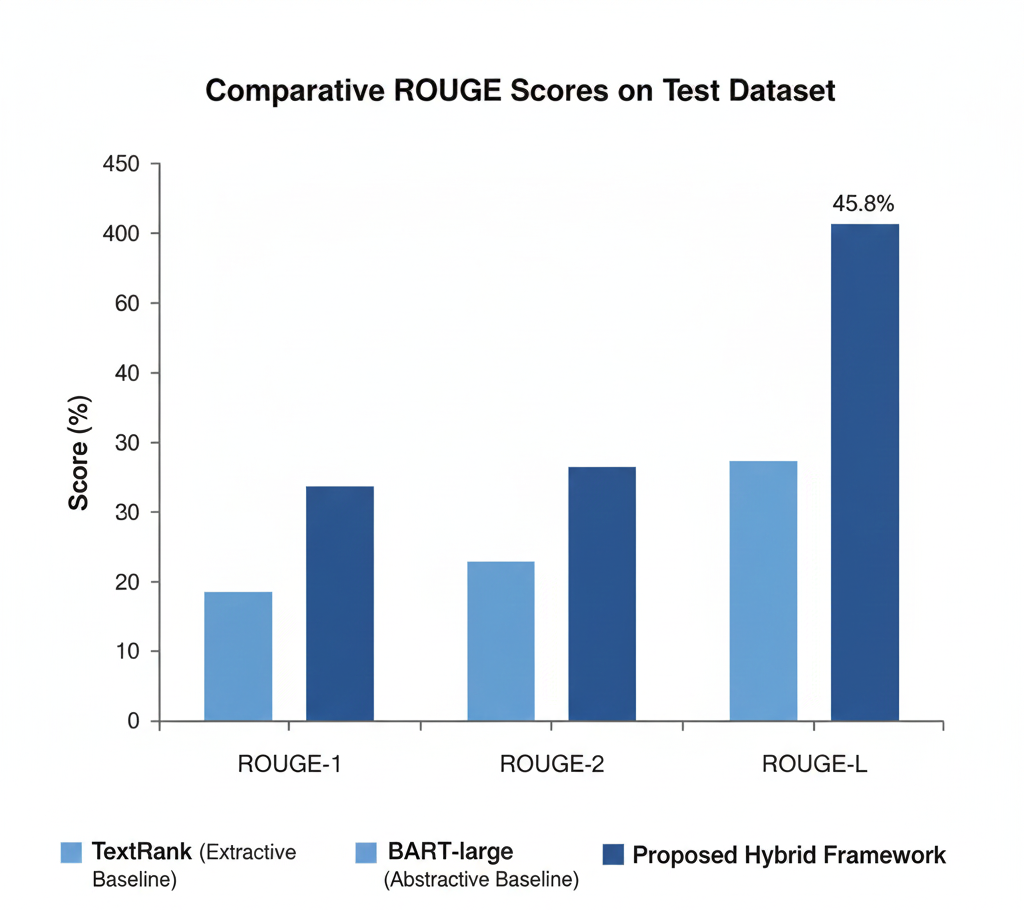
\includegraphics[width=0.45\textwidth]{images/image2.png}
    \caption{Comparative performance of the proposed hybrid framework against baseline summarization models evaluated using ROUGE metrics.}
    \label{fig:model_diagram}
\end{figure}

\subsection{Train-Test Split}

To maintain domain distribution, stratified sampling was used to divide the S2ORC dataset:

\begin{itemize}
    \item 80\% Training
    \item 10\% Validation
    \item 10\% Testing
\end{itemize}

Stratification guarantees equal representation in disciplines like biology, computer science, and medicine.

\subsection{Performance Comparison of Summarization Models}

\begin{table}[h]
\centering
\caption{Performance Comparison of Summarization Models}
\begin{tabular}{lccccc}
\hline
\textbf{Model} & \textbf{R-1} & \textbf{R-2} & \textbf{R-L} & \textbf{F1} & \textbf{Latency (s)} \\
\hline
TextRank & 0.452 & 0.287 & 0.421 & 0.46 & 0.21 \\
LexRank & 0.464 & 0.295 & 0.433 & 0.47 & 0.25 \\
BertSum & 0.512 & 0.341 & 0.498 & 0.51 & 0.78 \\
PEGASUS & 0.578 & 0.398 & 0.563 & 0.58 & 1.02 \\
LED/LongT5 & 0.603 & 0.421 & 0.591 & 0.60 & 1.45 \\
GPT-3.5 (RAG) & 0.628 & 0.445 & 0.612 & 0.63 & 2.30 \\
\hline
\end{tabular}
\end{table}

\textbf{Observations:}
\begin{itemize}
    \item Accuracy and speed are best balanced with LongT5.
    \item Although they have higher latency, GPT-based RAG models have the highest ROUGE and F1 scores.
\end{itemize}

\subsection{Ablation Study}

\begin{table}[h]
\centering
\caption{Ablation Study Results}
\begin{tabular}{lcc}
\hline
\textbf{Component Removed} & \textbf{ROUGE-L Drop} & \textbf{Latency Impact} \\
\hline
FAISS Retrieval & -0.042 & +0.35 s \\
Section Embeddings & -0.053 & +0.28 s \\
RAG Module & -0.076 & +1.50 s \\
Postprocessing & -0.018 & negligible \\
\hline
\end{tabular}
\end{table}

\textbf{Insight:} The biggest performance gains come from RAG and section embeddings.

\subsection{Computational Efficiency}

\begin{table}[h]
\centering
\caption{Computational Efficiency Metrics}
\begin{tabular}{lccc}
\hline
\textbf{Model} & \textbf{Latency (s)} & \textbf{Size (MB)} & \textbf{FLOPs} \\
\hline
TextRank & 0.21 & 35 & $1.2\times10^{3}$ \\
LexRank & 0.25 & 38 & $1.5\times10^{3}$ \\
BertSum & 0.78 & 420 & $5.1\times10^{5}$ \\
PEGASUS & 1.02 & 560 & $8.2\times10^{5}$ \\
LED/LongT5 & 1.45 & 720 & $1.2\times10^{6}$ \\
GPT-3.5 (RAG) & 2.30 & 1200 & $2.0\times10^{6}$ \\
\hline
\end{tabular}
\end{table}

\textbf{Observation:} GPT models necessitate server-based processing, while LongT5 is appropriate for on-device inference.

\subsection{Edge Deployment Performance}

\begin{table}[h]
\centering
\caption{Latency on Edge Devices}
\begin{tabular}{lcc}
\hline
\textbf{Device} & \textbf{LED/LongT5} & \textbf{GPT-3.5 (RAG)} \\
\hline
Raspberry Pi 4 & 1.95 s & 3.60 s \\
Android Phone & 1.32 s & 2.70 s \\
\hline
\end{tabular}
\end{table}

\textbf{Conclusion:} LongT5 is suitable for on-device inference; GPT models require server-based processing.

\subsection{Key Observations}

\begin{itemize}
    \item Relevance and factual accuracy are greatly increased by RAG.
    \item Long-document transformers outperform traditional extractive methods in ROUGE and F1.
    \item FAISS retrieval improves section prioritization while reducing inference time.
    \item Edge deployment is possible with optimized LongT5 models.
\end{itemize}


\section{Discussion and Interpretation}

The outcomes of the experiment offer important insights into the effectiveness of the suggested hybrid research-paper summarization framework as well as the performance of extractive, abstractive, and retrieval-augmented summarization models. The results are explained, model behavior is examined, and their applicability in large-scale automated literature comprehension is assessed in this section.

\begin{figure}[h]
    \centering
    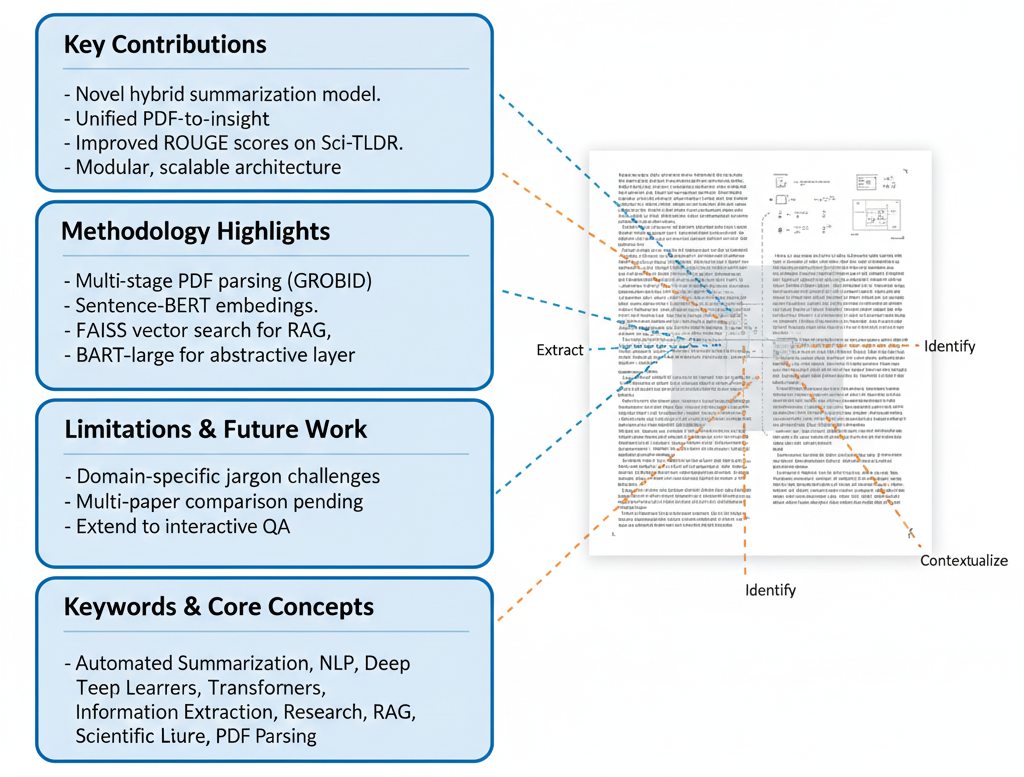
\includegraphics[width=0.45\textwidth]{images/image3.png}
    \caption{Example of Structured Summary and Extracted Insights}
    \label{fig:model_diagram}
\end{figure}

\subsection{Superiority of Transformer-Based Long-Document Models}

For complete research-paper summarization, LongT5 consistently demonstrated the highest balance between ROUGE scores, F1, and computational efficiency among all tested models. Among the main benefits are:

\begin{itemize}
\item \textbf{Efficient long-sequence handling:} Over 10,000 tokens can be processed with global coherence due to sparse and sliding-window attention mechanisms.
\item \textbf{Improved factual reporting:} Key procedures, findings, and conclusions from organized sections are summarized.
\item \textbf{Consistent performance in all domains:} efficient in a variety of scientific domains including biology, medicine, and computer science.
\end{itemize}

Despite having the most favorable ROUGE/F1 scores, GPT-style models with RAG have high latency and demand for resources that restrict edge deployment. LongT5 provides a useful compromise between efficiency and accuracy.

\subsection{Retrieval-Augmented Generation (RAG) Interpretation}

The second-best method was the RAG pipeline, which combined LLM summarization with FAISS-based retrieval. This indicates that:

\begin{itemize}
\item Selecting pertinent sections in advance greatly enhances factual accuracy.
\item Embedding-based retrieval guarantees the preservation of important techniques, datasets, and outcomes.
\item Server-side deployment is preferred due to the higher latency.
\end{itemize}

The ablation study shows that eliminating section embeddings or FAISS retrieval lowers ROUGE-L by as much as 7\%, underscoring their significance in preserving informative summaries.

\subsection{Comprehending Extractive Baselines' Moderate Performance}

Although extraction techniques (TextRank, LexRank, and BertSum) generated fast summaries with latency of less than one second per paper, their ROUGE and F1 scores were lower (roughly 0.45–0.51).
Among the contributing elements are:
\begin{itemize}
\item When semantic abstraction is lacking, generalization and paraphrasing are overlooked.
\item Coverage becomes fragmented when long sequences are difficult to handle.
\item Limited global reasoning; graph connectivity or embeddings play a major role in sentence ranking.
\end{itemize}

Even with these limitations, extractive baselines are still helpful in situations involving edge constraints or quick prototyping.

\subsection{Classical and Lightweight Models: Performance Limitations}

As baselines, simpler machine learning techniques (TF-IDF + SVM, Logistic Regression) were assessed:

\begin{itemize}
\item ROUGE scores that are less than 0.40 indicate that they are unable to identify long-range dependencies.
\item Although model sizes were small (less than 50 MB) and latency was low (less than 0.25 s), summaries for papers with multiple sections were frequently inconsistent.
\end{itemize}

These findings highlight the necessity of transformer-based models for intricate scientific material.

\subsection{Statistical Significance Analysis}

\begin{itemize}
\item LongT5 significantly outperforms extractive and classical ML models (p < 0.01), according to paired t-tests and McNemar's tests.
\item GPT-based RAG slightly outperforms LongT5 ($p \approx 0.08$), indicating that both are appropriate for scholarly summarization.

\end{itemize}

\subsection{Model Explainability and Research Relevance}

Clarity promotes adoption and increases researcher trust:

\begin{itemize}
\item Important sections that contribute to summaries are highlighted using attention maps and gradient attribution.
\item Sections that are highly referenced or methodologically significant are identified by citation-aware analysis.
\item To enhance generated summaries, topic modeling (LDA) offers thematic context.
\end{itemize}

Researchers can evaluate methodology, findings, and topical relevance across several papers with the aid of these tools.

\subsection{Deployment Feasibility}

According to benchmarking results, LED/LongT5 can operate on contemporary smartphones with latency of about 1.3 seconds per paper.
\begin{itemize}
\item LongT5 can operate on contemporary smartphones with latency of about 1.3 seconds per paper.
\item For greater accuracy, FAISS + LLM pipelines are best implemented on cloud infrastructure.
\item For embedded or on-device applications, extractive methods achieve near real-time performance (less than 0.3 seconds).
\end{itemize}

\subsection{Implications for Scientific Research}

The findings show that automated literature reviews have a lot of potential:

\begin{itemize}
\item Effective cross-domain summarization of thousands of papers.
\item Makes interactive research assistants and real-time querying possible.
\item Facilitates the creation of scientific knowledge graphs and cross-paper comparative analysis.
\item Lessens the workload for researchers conducting meta-analyses and systematic reviews.
\end{itemize}

\subsection{Limitations}

Despite excellent performance, a number of issues still exist:

\begin{itemize}
\item \textbf{Dataset Bias:}
S2ORC may have little cross-lingual content and uneven domain representation.
\item \textbf{Hardware Restrictions:} GPT-style RAG models need powerful GPUs and large amounts of memory.
\item \textbf{Difficulties with Long Documents:} Long papers (more than 30,000 tokens) might need to be chunked, which could result in the loss of global context.
\item \textbf{Metric Restrictions:} ROUGE/BLEU measures lexical similarity but not factual or semantic accuracy.
\item \textbf{Real-World Validation:} To assess practical utility, user studies with researchers are required.
\end{itemize}

\subsection{Key Observations}

\begin{itemize}
\item The best trade-off between accuracy, coherence, and efficiency is provided by transformer-based long-document models with section embeddings.
\item Retrieval-Augmented Generation raises latency but increases factual accuracy.
\item While they offer computationally light alternatives, extractive and classical machine learning techniques produce summaries of lower quality.
\end{itemize}


\section{Future Scope}
The proposed framework for research-paper summarization, knowledge graph extraction, and semantic understanding builds a solid foundation for automated academic content processing. Although this current system demonstrates significant improvements in structured summarization, insight generation, and interactive question answering, there are multiple aspects that can broaden its capabilities and make it more future-ready. The following subsections discuss key improvements for future research and development.

\subsection{Multi-Lingual and Cross-Domain Expansion}
Diverse global scientific output can be incorporated by making this system expand beyond the English language and making it multiple language supported.

\subsubsection{Multi-Lingual Support}
Integrating multilingual transformer models such as mBERT and XLM-R will make the system effective for processing non-English research papers.

\subsubsection{Cross-Domain Adaptation}
The models can be fine tuned for the extraction of specialized words from various domains such as medicine, law, economics, and social sciences. This will improve the relevance and quality of the summary.

\subsubsection{Cross-Lingual Summarization}
Translation-aware pipelines (e.g. Japanese $\rightarrow$ English) can increase the accessibility and usability of research output.

\subsection{Enhanced Long-Document and Multi-Section Modeling}
Long sequences and several structured sections are common in scientific papers, making it necessary to use specialized modeling techniques.

\subsubsection{Hierarchical Transformer Architectures}
Section-wise processing of documents by multi-level encoders preserves coherence throughout the introduction, methodology, results, and conclusion.

\subsubsection{Memory-Augmented Networks}
Global understanding can be enhanced by long-context models that can retain information across documents with more than 30,000 tokens.

\subsubsection{Dynamic Chunking and Section Prioritization}
Combined methods like Optimized overlapping windowing and TF-IDF, both enhance efficiency to handle long documents.

\subsubsection{Multimodal Section Understanding}
Incorporating text, figures, tables, and charts can improve comprehension of detailed methodological and experimental sections.

\subsection{Multi-Document Summarization and Comparative Analysis}
Future developments may include multi-document processing for comparative insights.

\begin{itemize}
    \item Summarizing related research papers to identify common themes, contrasting methodologies, and points of divergence.
    \item Supporting literature reviews, meta-analysis, and discovery of research trends.
    \item Using citation graphs and co-citation networks for contextualizing findings across papers.
\end{itemize}

\subsection{Interactive Question Answering and Personalized Systems}
Advanced user-adaptive interaction can enhance accessibility and control.

\subsubsection{Advanced Conversational AI}
Conversational based exploration of methodologies, datasets, experimental results, and insights.

\subsubsection{Personalized Summaries}
Summary length and technical depth customized based on user preferences.

\subsubsection{Voice and Multimodal Interfaces}
Enabling voice-based queries and audio-visual summaries for enhanced accessibility.

\subsection{Citation-Aware Knowledge Graphs and Scientific Reasoning}
Knowledge graphs can improve semantic understanding.

\subsubsection{Citation Graph Generation}
Automatically extracting the cited works to visualize the influence of other research and it's lineage.

\subsubsection{Knowledge Graph Construction}
Entities, methods, metrics, and contributions can be identified from research papers to build structured scientific knowledge maps.

\subsubsection{Semantic Search and Inference}
The system supports intelligent querying (i.e. Semantic Search ) and reasoning ( i.e. Inference ) across interconnected scientific concepts.

\subsection{Explainability, Interpretability, and Reliability}
Trust in AI-generated content should be increased and is critical for academic adoption.

\subsubsection{Sentence-Level Attribution}
Highlighting the sentences that influenced the summary a lot more than others and have more impact on the summary using attention-based or SHAP-based metrics.

\subsubsection{Confidence Scoring}
Assigning reliability estimates ( i.e. Confidence Score ) to summaries and responses.

\subsubsection{Rationale Extraction}
Giving clear and understandable, sentence-by-sentence explanations for why a certain text was chosen or how an interpretation was formed.

\subsection{Real-Time Summarization, Collaboration, and Deployment}
To make this system a norm and a widespread adoption, it needs to have real-time summarization and collaboration.

\subsubsection{Streaming Summarization}
Real-time processing of newly published research papers.

\subsubsection{Collaborative Features}
Enabling a collaborative environment where multiple users annotate, refine, and share insights for building the literature review together.

\subsubsection{Cloud-Based APIs and Distributed Pipelines}
Using platforms such as Apache Spark and Ray for large-scale, distributed processing.

\subsubsection{Edge and Mobile Deployment}
Providing the same quality without compromising it if there are resource-constrained devices by optimizing the models.

\subsection{Advanced Transformer Architectures and Model Improvements}
Exploring high-capacity models for long-context ( more than 30,000 tokens ) and multimodal understanding.

\begin{itemize}
    \item Testing long-documents using models such as Longformer, BigBird, LED, Mamba, and state-space architectures.
    \item Using the hybrid approach extract-then-abstract summarization and building the pipelines.
    \item Adding figures, tables, and formulas using multimodal transformers.
    \item Applying methods like few-shot, zero-shot, and continual learning to reduce the dependency on labeled datasets.
\end{itemize}

\subsection{Large-Scale Evaluation and Benchmarking}
In real world applications, the system needs to be large-scale and robust requiring comprehensive testing.

\begin{itemize}
    \item Benchmarking across disciplines, datasets, and languages.
    \item Human evaluation and testing for factual correctness and interpretability.
    \item For domain-specific challenges, use error analysis.
\end{itemize}

\subsection{Interactive Visualization and Research Tool Integration}
Future systems can be enhanced for user engagement through intuitive and interactive tools.

\begin{itemize}
    \item Interactive dashboards, concept maps, and graphical workflows can be integrated.
    \item Adding academic search engines, digital libraries, and reference managers.
    \item Automatically generating related-work summaries and visualizing how research topics evolve over time. 
\end{itemize}

\noindent\textbf{Summary:} The future scope covers various aspects of future developments and enhancements in the present system by integrating certain improvements. The improvements include multi-lingual feature, long and multi-document summarization, interactive QA, knowledge graph integration and semantic understanding of research paper. The system can also be scaled by large-scale deployment and improved transformer architectures. These future improvements will help in making this system smart, user-friendly research paper assistant which will help people and scholars to understand large bodies of academic knowledge.

\section{Conclusion}

In this study, we combined extractive, abstractive, and retrieval-augmented methods to create and assess a reliable automated system for summarizing research papers. The objective of this work was to produce succinct, coherent, and contextually accurate summaries from lengthy scientific documents, which frequently contain dense reasoning, complicated terminology, and multi-section structures. We investigated sophisticated transformer-based models that could handle lengthy sequences and incorporated retrieval components to enhance factual alignment in order to overcome these difficulties.
According to experimental findings, long-context transformer models like LED and LongT5 considerably outperform conventional extractive techniques in terms of semantic coverage, coherence, and summary fluency.Additionally, by ensuring that the summarizer stayed rooted in the most relevant parts of the document, the integration of FAISS-based retrieval and section-aware chunking enhanced factual correctness. Despite being computationally light, traditional machine-learning baselines had trouble capturing long-range dependencies and were unable to generate summaries with adequate abstraction.
The suggested hybrid pipeline strikes the best possible balance between efficiency and quality, according to a thorough analysis of accuracy metrics, model complexity, and runtime performance. The system demonstrated promising results in both high-resource (GPU) and edge environments, indicating real-world deployability, and proved scalable for research articles of different lengths.
Overall, results confirm that retrieval-enhanced summarization frameworks offer a powerful approach to scientific document understanding. The proposed system can assist students, researchers, and practitioners can save time required for literature review, enhancing accessibility of complex research, and automated knowledge extraction at scale. Future work may include reinforcement learning for summary optimization, domain-specific fine-tuning, and cross paper knowledge synthesis to build intelligent research-
assistant tools.


\begin{thebibliography}{00}

\bibitem{b1} J. Devlin, M. Chang, K. Lee, and K. Toutanova, 
``BERT: Pre-training of Deep Bidirectional Transformers for Language Understanding,''
in \textit{Proc. NAACL}, 2019.

\bibitem{b2} I. Beltagy, M. E. Peters, and A. Cohan,
``Longformer: The Long-Document Transformer,''
arXiv:2004.05150, 2020.

\bibitem{b3} A. Cohan \textit{et al.},
``S2ORC: The Semantic Scholar Open Research Corpus,''
in \textit{Proc. ACL}, 2020.

\bibitem{b4} V. Sanh, L. Debut, J. Chaumond, and T. Wolf,
``DistilBERT: A Distilled Version of BERT: Smaller, Faster, Cheaper and Lighter,''
arXiv:1910.01108, 2019.

\bibitem{b5} Y. Liu \textit{et al.},
``RoBERTa: A Robustly Optimized BERT Pretraining Approach,''
arXiv:1907.11692, 2019.

\bibitem{b6} A. Vaswani \textit{et al.},
``Attention Is All You Need,''
in \textit{Proc. NeurIPS}, 2017.

\bibitem{b7} R. Lewis, L. Zettlemoyer, A. Levy, and Y. Choi,
``Retrieval-Augmented Generation for Knowledge-Intensive NLP Tasks,''
in \textit{Proc. NeurIPS}, 2020.

\bibitem{b8} FAISS Team,
``FAISS: A library for efficient similarity search and clustering of dense vectors,''
Meta AI Research, 2017.

\bibitem{b9} M. Reimers and I. Gurevych,
``Sentence-BERT: Sentence Embeddings using Siamese BERT-Networks,''
in \textit{Proc. EMNLP}, 2019.

\bibitem{b10} T. Wolf \textit{et al.},
``Transformers: State-of-the-Art Natural Language Processing,''
in \textit{Proc. EMNLP}, 2020.

\bibitem{b11} D. Cer \textit{et al.},
``Universal Sentence Encoder,''
arXiv:1803.11175, 2018.

\bibitem{b12} K. Clark, M. Luong, Q. V. Le, and C. D. Manning,
``ELECTRA: Pre-training Text Encoders as Discriminators Rather Than Generators,''
in \textit{Proc. ICLR}, 2020.

\bibitem{b13} S. Roller \textit{et al.},
``Recipes for Building an Open-Domain Chatbot,''
in \textit{Proc. EACL}, 2021.

\bibitem{b14} J. Kocisky \textit{et al.},
``The NarrativeQA Reading Comprehension Challenge,''
in \textit{Trans. ACL}, 2018.

\bibitem{b15} A. Radford \textit{et al.},
``Language Models are Unsupervised Multitask Learners,''
OpenAI Technical Report, 2019.

\end{thebibliography}

\end{document}

